\subsection{Raspberry PI}
\label{sec:raspberry_pi}

Raspberry PIs sind eine Familie an \ac{SBC} welche von der Raspberry PI Foundation entwickelt und verkauft werden. Die \ac{Arm} basierten Computer haben etwa die Grundflache einer Kreditkarte und sind etwa 2 cm hoch. Trotz ihrer Größe haben sie eine achtbare Rechenkapazität (neuere Modelle sogar bis zu 8 GB \ac{RAM} \citev{raspberry_pi_4b}). Dank der vielen Peripheriegeräte, wie \ac{GPIO}, \ac{SPI} und \ac{I2C} sind diese kleinen Computer ideal für das Steuern von Hardware und \ac{IoT} Anwendungen.

\begin{figure}[H]
  \centering
  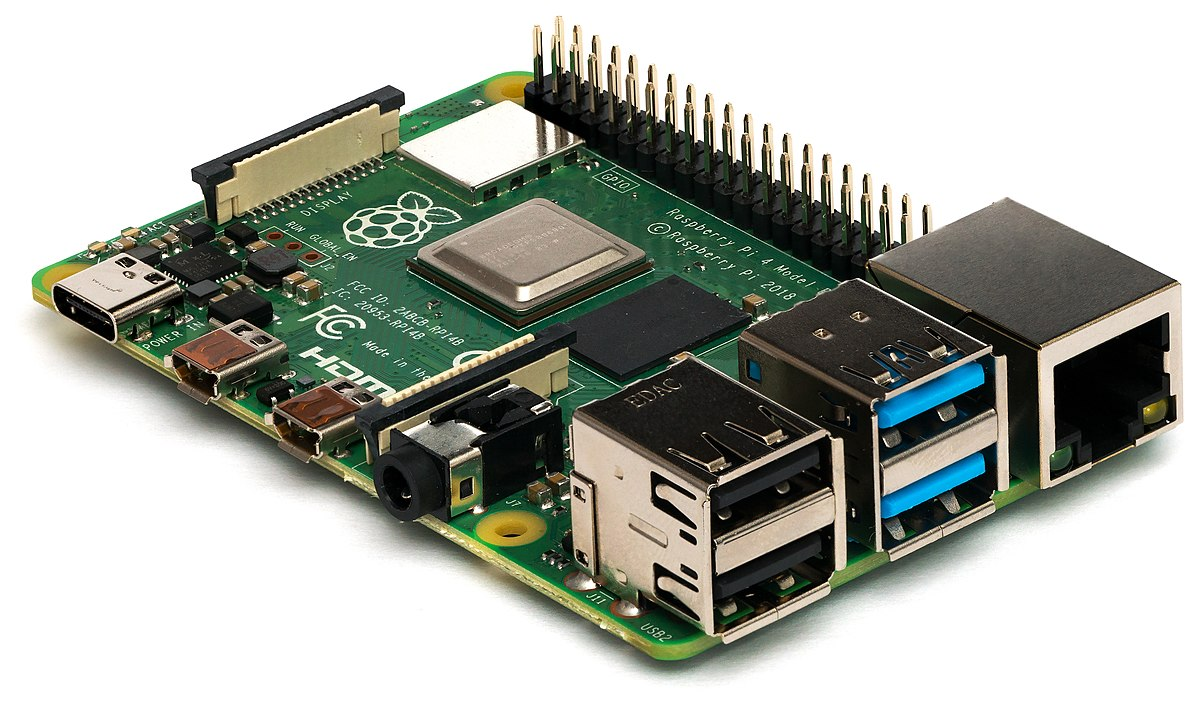
\includegraphics[width=0.75\textwidth]{images/raspberry_pi_4b}
  \caption{Raspberry PI 4b \citev{raspberry_pi_4b}}
  \label{fig:raspberry_pi_4b}
\end{figure}

Anders als wie bei Mikrocontrollern muss sich der Entwickler bei einem Raspberry PI nicht um alles kümmern. Zwischen Hardware und Software gibt es einen Kernel und ein Linux Betriebssystem, diese übernehmen viele der Aufgaben und erleichtern die Entwicklung. Somit ist es zum Beispiel möglich eine Python Applikation auf dem Raspberry PI auszuführen.

